The Ramsey Theorem brought to light and formalized an important property of graphs  directly related to how much they can grow when new vertices are added. A graph $G$ is called Ramsey big for a set of colors \colorset and a graph $H$ if any edge coloring of $G$ using \colorset has a monochromatic copy of $H$ as a subgraph. $G = $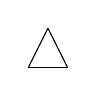
\begin{tikzpicture}[scale=0.5]
	\draw (0,0) -- (0.5,1);
	\draw (0,0) -- (1,0);
	\draw (0.5,1) -- (1,0);	
\end{tikzpicture} is big for $H = $
\begin{tikzpicture}[scale=0.5]
\draw (1,0) -- (0.5,1);
\end{tikzpicture}
using two colors. In the example, however it is possible to take edges of $G$ so that it remains big. $G =\;$
\begin{tikzpicture}[scale=0.5]
\draw (0.5,1) -- (1,0);
\draw (0,0) -- (1,0);
\end{tikzpicture}
and $G = $
\begin{tikzpicture}[scale=0.5]
\draw (1,0) -- (0.5,1);
\end{tikzpicture} are both big. The number of vertices of the smallest big graph is called Ramsey Graph Number. The example given is denoted by \ramGraph{H,H}.

More generally, however, each color can have its own target graph $H_{c_i}$ so the notation used is \ramGraph{H_1,\ldots,H_{|\colorset|}}.
However, in the special case that every target is a complete graph $K_{n_i}$, the amount of vertices in the smallest possible big graph is called Ramsey Number, instead of Ramsey Graph Number, and is denoted by $R(n_1, \ldots, n_{|\colorset|})$. 

The existence of big graphs for all target graphs and sets of colors is known since 1928 \todo{CITE On a problem of formal logic}, but the algebraic and computational challenges are yet to be solved. Ramsey Theory has many focuses of research, but one, is special, tends to the importance of knowing $G$ before the coloring process starts. That segment is called Online Ramsey Theory.

\subsection*{Online algorithms}

A well known online algorithm is the Canadian Traveler Problem. One tries to move from one city to another with bad whether conditions, making the connecting roads unpredictable. Using graph theoretical vocabulary, it is the problem of finding the shortest path between two vertices in a weighted directed graph, with one additional detail. At each step starting from the initial position, only the weight of the outgoing edges of the current vertex are known. That causes differences in the problem complexity when compared to the offline version solvable by Dijkstra's algorithm. 

\subsection*{Online Ramsey Theory}

The online version of the graph coloring problem studied in Ramsey theory is presented in different ways. Consider the following versions:

\begin{version}{1}
:Take a graph $G = K_n$ and a target $H$. Left and Right alternate coloring the edges of $K_n$ blue and red, respectively. The first player to create a monochromatic copy of $H$ in $G$ wins. If neither player is able to create it and there are no more uncolored edges, the game is a tie.
\end{version}

\begin{version}{2}
:Take a graph $G$ with no edges and a target $H$. Left selects two disconnected vertices of $G$ and adds an edge between them. Following, Right decides with what color to paint that edge. If a monochromatic copy of $H$ is ever created, then Left wins. It is common to allow $G$ to have an infinite amount of vertices, and consider that Right only wins if it provides a strategy to avoid $H$ indefinitely. In this version, Left and Right are typically called Builder and Painter, respectively.
\end{version}

Both versions are online as decisions are taken, either selecting, building or coloring edges, without knowledge of their consequences. For the remainder of this text version number two will be used and that is a matter of better matching the reference texts. Online algorithmic versions of the problem are typically referred to as Ramsey Games, Online Ramsey Theory and Online Ramsey Games.

The impact of the lack of information in the online version of the problem is significant. Pavel Dvo\v{r}\'ak shows in his master thesis \todo{cite his thesis} a very nice example, that was within reach since 2004, when the base theorem was proved in the paper ``On-line Ramsey Theory" \todo{cite text -> is in proposal too}. Consider the target is $P_3 = $
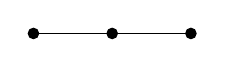
\begin{tikzpicture}
\begin{scope} [every node/.style={scale=0.4, circle, draw, fill=black}]
	\node (p1) at (0,0){};
	\node (p2) at (1,0){};
	\node (p3) at (2,0){};
\end{scope}
\draw (p1) -- (p2);
\draw (p2) -- (p3);
\end{tikzpicture}
. Now take $G =$
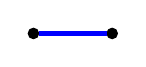
\begin{tikzpicture}
	\begin{scope} [every node/.style={scale=0.4, circle, draw, fill=black}]
		\node (p1) at (0,0){};
		\node (p2) at (1,0){};
	\end{scope}
	\draw[blue, ultra thick] (p1) -- (p2);
\end{tikzpicture}
. It is clear that in the next iteration $G^{LR} = G_1 =$
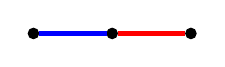
\begin{tikzpicture}
\begin{scope} [every node/.style={scale=0.4, circle, draw, fill=black}]
	\node (p1) at (0,0){};
	\node (p2) at (1,0){};
	\node (p3) at (2,0){};
\end{scope}
\draw[blue, ultra thick] (p1) -- (p2);
\draw[red, ultra thick] (p2) -- (p3);
\end{tikzpicture}
. Since $G_1$ is reachable, then so are  \hbox{$G_2 =$
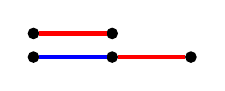
\begin{tikzpicture}
	\begin{scope} [every node/.style={scale=0.4, circle, draw, fill=black}]
		\node (p1) at (0,0){};
		\node (p2) at (1,0){};
		\node (p3) at (2,0){};
		\node (p4) at (0,0.3){};
		\node (p5) at (1,0.3){};
	\end{scope}
	\draw[blue, ultra thick] (p1) -- (p2);
	\draw[red, ultra thick] (p2) -- (p3);
	\draw[red, ultra thick] (p4) -- (p5);
\end{tikzpicture}}
and $G_3 =$
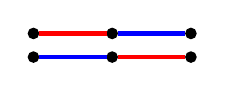
\begin{tikzpicture}
	\begin{scope} [every node/.style={scale=0.4, circle, draw, fill=black}]
		\node (p1) at (0,0){};
		\node (p2) at (1,0){};
		\node (p3) at (2,0){};
		\node (p4) at (0,0.3){};
		\node (p5) at (1,0.3){};
		\node (p6) at (2,0.3){};
	\end{scope}
	\draw[blue, ultra thick] (p1) -- (p2);
	\draw[red, ultra thick] (p2) -- (p3);
	\draw[red, ultra thick] (p4) -- (p5);
	\draw[blue, ultra thick] (p5) -- (p6);
\end{tikzpicture}
. Finally, by connecting either the left or the right ends of the two components, \hbox{$G^L_3 =$

\begin{tikzpicture}
	\begin{scope} [every node/.style={scale=0.4, circle, draw, fill=black}]
		\node (p1) at (0,0){};
		\node (p2) at (1,0){};
		\node (p3) at (2,0){};
		\node (p4) at (0,0.3){};
		\node (p5) at (1,0.3){};
		\node (p6) at (2,0.3){};
	\end{scope}
	\draw[blue, ultra thick] (p1) -- (p2);
	\draw[red, ultra thick] (p2) -- (p3);
	\draw[red, ultra thick] (p4) -- (p5);
	\draw[blue, ultra thick] (p5) -- (p6);
	\draw[ultra thick, darkgray] (p3) to[out=3,in=-3, distance=1cm] (p6);
\end{tikzpicture}}.
In $G_4$, the gray edge would be colored either blue nor red. Therefore, Left would win. However,consider the following recoloring of \hbox{$G_4$, $G^*_4 = $

\begin{tikzpicture}
	\begin{scope} [every node/.style={scale=0.4, circle, draw, fill=black}]
		\node (p1) at (0,0){};
		\node (p2) at (1,0){};
		\node (p3) at (2,0){};
		\node (p4) at (0,0.3){};
		\node (p5) at (1,0.3){};
		\node (p6) at (2,0.3){};
	\end{scope}
	\draw[blue, ultra thick] (p1) -- (p2);
	\draw[red, ultra thick] (p2) -- (p3);
	\draw[blue, ultra thick] (p4) -- (p5);
	\draw[red, ultra thick] (p5) -- (p6);
	\draw[blue, ultra thick] (p3) to[out=3,in=-3, distance=1cm] (p6);
\end{tikzpicture}}. 

What prevented Right from getting that valid recoloring instead of the defeat in $G_4$ was not knowing Left's next moves. If Right knew Left would connect the right corners of the two stripes from the beginning, then Right would have colored the top edge, in $G^L_2$, blue and not red.

\subsection*{Restricting G}

The main challenge and focus of study in Ramsey Theory is finding Ramsey numbers. A challenge in Online Ramsey Games is, similarly, finding the smallest number of turns necessary for Left to win. However, there are other questions like the minimum number of edges a graph must have in order to be big as well or finding required substructures. An additional source of problems, in both areas, is deciding the outcomes of restricting the domain to particular classes of graphs. 

As per the first part of the introduction, it is true that there exists a big graph $G$ for every target $H$ and color set \colorset in Ramsey games. Consider, on the other hand, the class $\mathcal{G}$ to be the class of bipartite graphs. If Left can only build graphs in $\mathcal{G}$, then a triangle would, of course, be unreachable, therefore it does not have big graphs. However, knowing whether every bipartite graph is unavoidable or, equivalently, knowing if $\mathcal{G}$ is self-unavoidable, makes up a harder problem.

\subsection*{Planar Graphs}

Graphs that can be drawn without crossing edges form a class that is most typical of graph theory. Without the crossing edges, graph images becomes much easier to parse and that makes up for great visualization handicaps. They form a specially nice class instance for Ramsey games because, although these games are mostly concerned with combinatorial and computational questions, visualizing them allows both human interaction and algorithm inspection.

Over the past twenty years great progress has been made in terms of finding self-unavoidable sub-classes and discovering more of the overall impacts this restriction causes to Ramsey games. The next sections of the text focus on bringing initial results and recent developments for planar graphs. Following, a new game will be proposed.













